\section{Auswertung}
\label{sec:Auswertung}

\begin{table}
  \centering
  \caption{Messung der Biegung des zylindrigen Stabs bei einseitiger Einspannung}
  \label{tab:ecks}
  \sisetup{table-format=2.1}
  \begin{tabular}{S[table-format=4.0] S[table-format=4.0]}
    \toprule
    {$x \mathbin{/} \si{\milli\meter}$} & {$D(x) \mathbin{/} \si{\milli\meter}$}\\
    \midrule
    1000 & 0,28\\
    1250 & 0,35\\
    1500 & 0,36\\
    1750 & 0,45\\
    2000 & 0,51\\
    2250 & 0,62\\
    2500 & 0,78\\
    2750 & 0,93\\
    3000 & 1,16\\
    3250 & 1,34\\
    3500 & 1,58\\
    3750 & 1,78\\
    4000 & 2,07\\
    4250 & 2,30\\
    4500 & 2,58\\
    4750 & 2,79\\
    5000 & 3,10\\
    5250 & 3,48\\
    \bottomrule
  \end{tabular}
\end{table}

\begin{table}
  \centering
  \caption{Messung der Biegung des eckigen Stabs bei einseitiger Einspannung}
  \label{tab:ecks}
  \sisetup{table-format=2.1}
  \begin{tabular}{S[table-format=4.0] S[table-format=4.0]}
    \toprule
    {$x \mathbin{/} \si{\milli\meter}$} & {$D(x) \mathbin{/} \si{\milli\meter}$}\\
    \midrule
    1000 & 0,32\\
    1250 & 0,46\\
    1500 & 0,62\\
    1750 & 0,73\\
    
  \end{tabular}
\end{table}

\begin{figure}
  \centering
  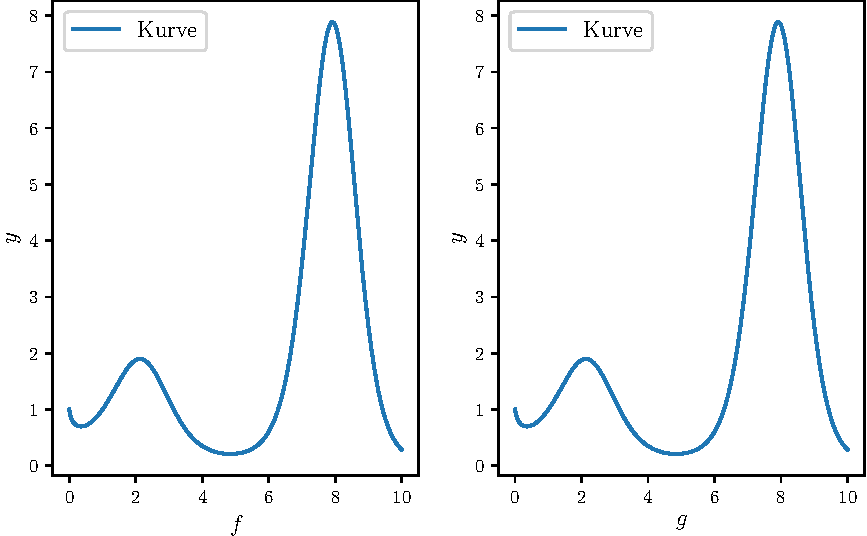
\includegraphics{plot.pdf}
  \caption{Plot.}
  \label{fig:plot}
\end{figure}


Siehe \autoref{fig:plot}!
